% TikZ figures for the referee reply. Requires: tikz with decorations.pathmorphing, arrows.meta
\tikzset{
  gluon/.style={decorate,decoration={coil,aspect=0.3,segment length=4.2pt,amplitude=2.6pt},thick},
  valence/.style={line width=1.8pt},
  cut/.style={dashed,gray!70!black},
  shell/.style={dashed,red!75!black,line width=1pt},
  lab/.style={font=\footnotesize},
  den/.style={font=\scriptsize,align=center},
}

%--------------------------------------------------------------------
\newcommand{\FigTchannel}{%
\begin{figure}[h!]
\centering
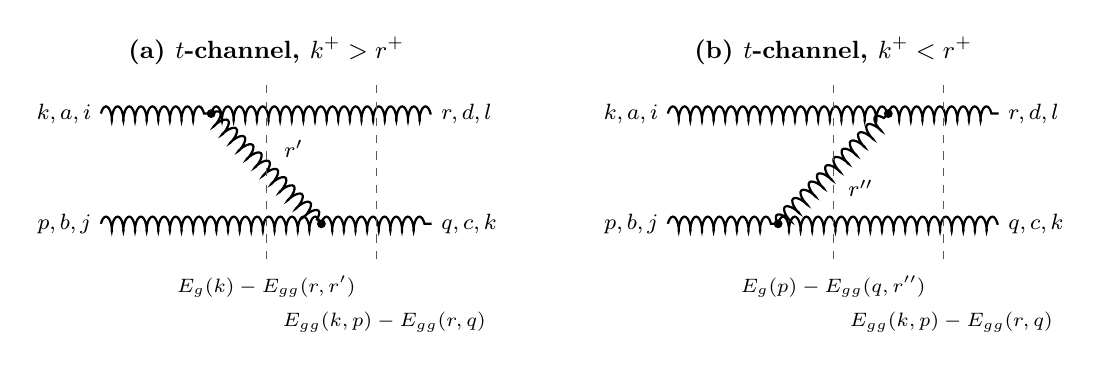
\begin{tikzpicture}[x=1cm,y=1cm]
% ---------- (a) t-channel, k emits ----------
\begin{scope}
 \draw[gluon] (0,1.4) -- (1.4,1.4);
 \draw[gluon] (1.4,1.4) -- (4.2,1.4);
 \draw[gluon] (0,0) -- (2.8,0);
 \draw[gluon] (2.8,0) -- (4.2,0);
 \draw[gluon] (1.4,1.4) -- (2.8,0);
 \fill (1.4,1.4) circle (1.6pt); \fill (2.8,0) circle (1.6pt);
 \node[lab,left] at (0,1.4) {$k,a,i$};
 \node[lab,left] at (0,0) {$p,b,j$};
 \node[lab,right] at (4.2,1.4) {$r,d,l$};
 \node[lab,right] at (4.2,0) {$q,c,k$};
 \node[lab] at (2.45,0.95) {$r'$};
 \draw[cut] (2.1,-0.45) -- (2.1,1.85);
 \draw[cut] (3.5,-0.45) -- (3.5,1.85);
 \node[den] at (2.1,-0.8) {$E_g(k)-E_{gg}(r,r')$};
 \node[den] at (3.6,-1.25) {$E_{gg}(k,p)-E_{gg}(r,q)$};
 \node[font=\small\bfseries] at (2.1,2.2) {(a) $t$-channel, $k^+>r^+$};
\end{scope}
% ---------- (b) t-channel, p emits ----------
\begin{scope}[xshift=7.2cm]
 \draw[gluon] (0,1.4) -- (2.8,1.4);
 \draw[gluon] (2.8,1.4) -- (4.2,1.4);
 \draw[gluon] (0,0) -- (1.4,0);
 \draw[gluon] (1.4,0) -- (4.2,0);
 \draw[gluon] (1.4,0) -- (2.8,1.4);
 \fill (2.8,1.4) circle (1.6pt); \fill (1.4,0) circle (1.6pt);
 \node[lab,left] at (0,1.4) {$k,a,i$};
 \node[lab,left] at (0,0) {$p,b,j$};
 \node[lab,right] at (4.2,1.4) {$r,d,l$};
 \node[lab,right] at (4.2,0) {$q,c,k$};
 \node[lab] at (2.45,0.45) {$r''$};
 \draw[cut] (2.1,-0.45) -- (2.1,1.85);
 \draw[cut] (3.5,-0.45) -- (3.5,1.85);
 \node[den] at (2.1,-0.8) {$E_g(p)-E_{gg}(q,r'')$};
 \node[den] at (3.6,-1.25) {$E_{gg}(k,p)-E_{gg}(r,q)$};
 \node[font=\small\bfseries] at (2.1,2.2) {(b) $t$-channel, $k^+<r^+$};
\end{scope}
\end{tikzpicture}

\vspace{10pt}
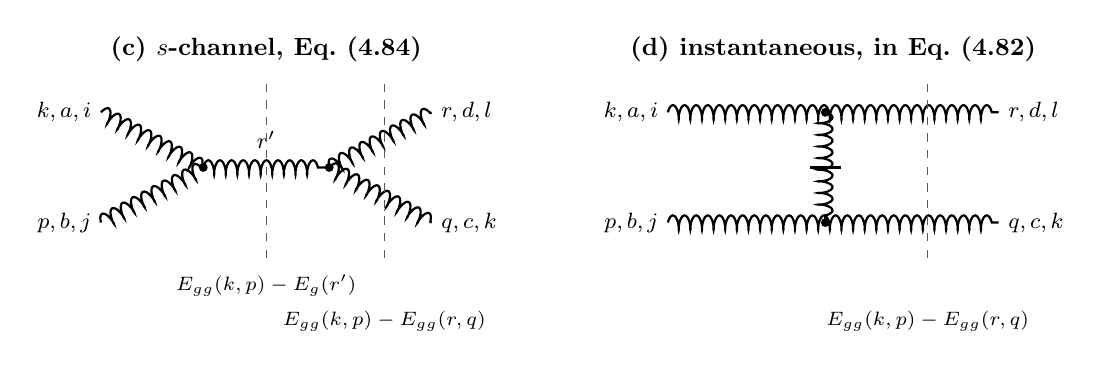
\begin{tikzpicture}[x=1cm,y=1cm]
% ---------- (c) s-channel (already in the paper) ----------
\begin{scope}
 \draw[gluon] (0,1.4) -- (1.3,0.7);
 \draw[gluon] (0,0) -- (1.3,0.7);
 \draw[gluon] (1.3,0.7) -- (2.9,0.7);
 \draw[gluon] (2.9,0.7) -- (4.2,1.4);
 \draw[gluon] (2.9,0.7) -- (4.2,0);
 \fill (1.3,0.7) circle (1.6pt); \fill (2.9,0.7) circle (1.6pt);
 \node[lab,left] at (0,1.4) {$k,a,i$};
 \node[lab,left] at (0,0) {$p,b,j$};
 \node[lab,right] at (4.2,1.4) {$r,d,l$};
 \node[lab,right] at (4.2,0) {$q,c,k$};
 \node[lab] at (2.1,1.05) {$r'$};
 \draw[cut] (2.1,-0.45) -- (2.1,1.85);
 \draw[cut] (3.6,-0.45) -- (3.6,1.85);
 \node[den] at (2.1,-0.8) {$E_{gg}(k,p)-E_{g}(r')$};
 \node[den] at (3.6,-1.25) {$E_{gg}(k,p)-E_{gg}(r,q)$};
 \node[font=\small\bfseries] at (2.1,2.2) {(c) $s$-channel, Eq.~(4.84)};
\end{scope}
% ---------- (d) instantaneous t-exchange (part of 4.82) ----------
\begin{scope}[xshift=7.2cm]
 \draw[gluon] (0,1.4) -- (4.2,1.4);
 \draw[gluon] (0,0) -- (4.2,0);
 \draw[gluon] (2.0,1.4) -- (2.0,0);
 \draw[thick] (1.8,0.7) -- (2.2,0.7);
 \fill (2.0,1.4) circle (1.6pt); \fill (2.0,0) circle (1.6pt);
 \node[lab,left] at (0,1.4) {$k,a,i$};
 \node[lab,left] at (0,0) {$p,b,j$};
 \node[lab,right] at (4.2,1.4) {$r,d,l$};
 \node[lab,right] at (4.2,0) {$q,c,k$};
 \draw[cut] (3.3,-0.45) -- (3.3,1.85);
 \node[den] at (3.3,-1.25) {$E_{gg}(k,p)-E_{gg}(r,q)$};
 \node[font=\small\bfseries] at (2.1,2.2) {(d) instantaneous, in Eq.~(4.82)};
\end{scope}
\end{tikzpicture}
\caption{Gluon exchange between two incoming soft gluons at $\mathcal O(g^2)$. Light-cone time runs from left to right; dashed vertical lines mark the intermediate and final states, with the corresponding energy denominators written below. Diagrams (a) and (b) are the two light-cone time orderings of the non-instantaneous $t$-channel exchange, which are missing from Sec.~4.3.1; their intermediate state has \emph{three} gluons. Plus-momentum positivity of the exchanged gluon ($r'^+=k^+-r^+>0$ in (a), $r''^+=r^+-k^+>0$ in (b)) means that exactly one of them contributes for given external momenta. The $u$-channel diagrams follow from $r\leftrightarrow q$. For comparison, (c) is the $s$-channel exchange already contained in Eq.~(4.84), and (d) is the instantaneous part of the $t$-channel exchange (crossed line), already contained in Eq.~(4.82).}
\label{fig:tchannel}
\end{figure}}

%--------------------------------------------------------------------
\newcommand{\FigShell}{%
\begin{figure}[h!]
\centering
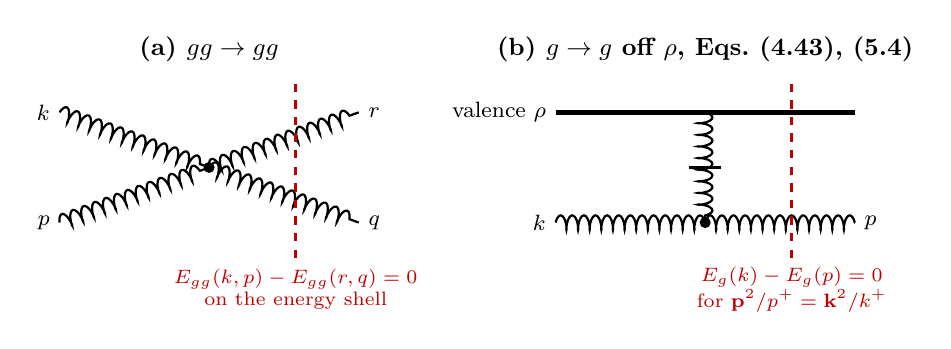
\begin{tikzpicture}[x=1cm,y=1cm]
% ---------- (a) 2 -> 2 with final-state cut ----------
\begin{scope}
 \draw[gluon] (0,1.4) -- (1.9,0.7);
 \draw[gluon] (0,0) -- (1.9,0.7);
 \draw[gluon] (1.9,0.7) -- (3.8,1.4);
 \draw[gluon] (1.9,0.7) -- (3.8,0);
 \fill (1.9,0.7) circle (2pt);
 \node[lab,left] at (0,1.4) {$k$};
 \node[lab,left] at (0,0) {$p$};
 \node[lab,right] at (3.8,1.4) {$r$};
 \node[lab,right] at (3.8,0) {$q$};
 \draw[shell] (3.0,-0.45) -- (3.0,1.85);
 \node[den,red!75!black] at (3.0,-0.85) {$E_{gg}(k,p)-E_{gg}(r,q)=0$\\ on the energy shell};
 \node[font=\small\bfseries] at (1.9,2.2) {(a) $gg\to gg$};
\end{scope}
% ---------- (b) 1 -> 1 off the valence background ----------
\begin{scope}[xshift=6.3cm]
 \draw[valence] (0,1.4) -- (3.8,1.4);
 \node[lab,left] at (0,1.4) {valence $\rho$};
 \draw[gluon] (0,0) -- (1.9,0);
 \draw[gluon] (1.9,0) -- (3.8,0);
 \draw[gluon] (1.9,1.4) -- (1.9,0);
 \draw[thick] (1.7,0.7) -- (2.1,0.7);
 \fill (1.9,0) circle (2pt);
 \node[lab,left] at (0,0) {$k$};
 \node[lab,right] at (3.8,0) {$p$};
 \draw[shell] (3.0,-0.45) -- (3.0,1.85);
 \node[den,red!75!black] at (3.0,-0.85) {$E_{g}(k)-E_{g}(p)=0$\\ for $\mathbf p^2/p^+=\mathbf k^2/k^+$};
 \node[font=\small\bfseries] at (1.9,2.2) {(b) $g\to g$ off $\rho$, Eqs.~(4.43), (5.4)};
\end{scope}
\end{tikzpicture}

\vspace{10pt}
\begin{tikzpicture}[x=1cm,y=1cm]
% ---------- (c) the energy shell in (xi', kappa') ----------
\begin{scope}
 \def\xin{0.3}\def\kin{1.0}
 \fill[red!8] (0,0) -- plot[domain=0:1,samples=80] ({5*\x},{2.2*\kin*sqrt(\x*(1-\x)/(\xin*(1-\xin)))}) -- (5,0) -- cycle;
 \draw[->] (0,0) -- (5.4,0) node[right,lab] {$\xi'=r^+/P^+$};
 \draw[->] (0,0) -- (0,3.1) node[above,lab] {$|\boldsymbol\kappa'|$};
 \draw[shell,solid] plot[domain=0:1,samples=80] ({5*\x},{2.2*\kin*sqrt(\x*(1-\x)/(\xin*(1-\xin)))});
 \fill (5*\xin,2.2*\kin) circle (2pt) node[above left,lab] {$(\xi,|\boldsymbol\kappa|)$};
 \draw (5,0) -- (5,-0.08) node[below,lab] {$1$};
 \node[lab] at (0,-0.25) {$0$};
 \node[lab,red!75!black] at (3.6,1.15) {$E_i>E_f$};
 \node[lab] at (3.9,2.85) {$E_i<E_f$};
 \node[font=\small\bfseries] at (2.6,3.55) {(c) energy shell of $gg\to gg$};
\end{scope}
% ---------- (d) complex x-plane ----------
\begin{scope}[xshift=9.4cm,yshift=1.3cm]
 \draw[->] (-2.2,0) -- (2.4,0) node[right,lab] {$\mathrm{Re}\,x$};
 \draw[->] (0,-1.5) -- (0,1.6) node[above,lab] {$\mathrm{Im}\,x$};
 \draw[very thick,blue!60!black,->] (-2,0.04) -- (-0.2,0.04);
 \draw[very thick,blue!60!black] (-0.2,0.04) -- (2.1,0.04);
 \node[lab,blue!60!black] at (1.3,0.3) {integration};
 \node[red!75!black] at (0,-0.9) {$\times$};
 \node[lab,red!75!black,right] at (0.1,-0.9) {$x=-2i\varepsilon$};
 \node[lab,align=left] at (0.3,-2.05) {$\dfrac{1}{x+2i\varepsilon}\;\to\;\mathrm P\dfrac1x-i\pi\delta(x)$};
 \node[font=\small\bfseries] at (0.1,2.25) {(d) prescription, $x=E_i-E_f$};
\end{scope}
\end{tikzpicture}
\caption{The vanishing energy denominator of Comment 2. (a)~Any $gg\to gg$ amplitude, whether contact, instantaneous, $s$- or $t$-channel, carries the overall denominator $E_{gg}(k,p)-E_{gg}(r,q)$ of the final state (red dashed cut). (b)~The same happens for gluon-number-preserving scattering off the valence background, e.g.\ the instantaneous term (4.43) and $\mathbb B_3$ in (5.4). (c)~With $\xi=k^+/P^+$ and $\boldsymbol\kappa=(1-\xi)\mathbf k-\xi\mathbf p$ fixed, the denominator vanishes on the curve $|\boldsymbol\kappa'|^2=|\boldsymbol\kappa|^2\,\xi'(1-\xi')/[\xi(1-\xi)]$ (red), which lies \emph{inside} the region of integration over the outgoing momenta; it separates configurations with $E_i>E_f$ (shaded) from those with $E_i<E_f$. (d)~The adiabatic switching of Eq.~(3.7) moves the pole to $x=-2i\varepsilon$ below the real axis at second order. As $\varepsilon\to0$ this gives a principal value, which is integrable, plus an on-shell $\delta$-function term.}
\label{fig:shell}
\end{figure}}
